\documentclass[letterpaper, 12pt]{report}
\usepackage[utf8]{inputenc}
\usepackage[english, spanish]{babel}
\usepackage{fullpage} 
\usepackage{graphicx}
\usepackage{enumitem}
\usepackage{chngcntr}
\usepackage{float}
\usepackage{hyperref} 
\counterwithin{figure}{section}
\renewcommand{\thesection}{\arabic{section}}
\renewcommand{\thesubsection}{\thesection.\arabic{subsection}}
\renewcommand{\baselinestretch}{1.5}
\begin{document}

\begin{titlepage}
	\centering
	
\includegraphics[width=0.3\textwidth]{eii_ulpgc.png}\par\vspace{1cm}
	{\scshape\LARGE Universidad de Las Palmas de Gran Canaria \par}
	\vspace{1cm}
	{\scshape\Large Programación de Aplicaciones Móviles Nativas \par}
	\vspace{.2cm}
    {\scshape\Large Accesibilidad y normativa. Análisis de aplicaciones.\par}
	\vspace{1cm}
	{\Large\bfseries Comparación de Arquitecturas de Software \par}
	\vspace{1cm}
	{\itshape Paula Rosa Rodríguez Morales \par}
        {\itshape Anna Sajdokova \par}
	\vfill
	{\large \today\par}
\end{titlepage}

\tableofcontents
\newpage

\section{Introducción}
En el desarrollo de aplicaciones móviles, la elección de una arquitectura adecuada es crucial para garantizar la escalabilidad, el mantenimiento del código y la eficiencia en el manejo de interacciones complejas con el usuario. Existen varias arquitecturas populares que permiten estructurar aplicaciones de manera efectiva, cada una con sus propias ventajas y desventajas. Entre las más utilizadas en la industria destacan MVC (Model-View-Controller), MVP (Model-View-Presenter) y MVVM (Model-View-ViewModel).

Este trabajo se centra en realizar un estudio comparativo entre estas tres arquitecturas, evaluando su estructura, nivel de acoplamiento, facilidad para realizar pruebas, curva de aprendizaje y escalabilidad. A través de este análisis, se busca identificar qué arquitectura resulta más adecuada según el contexto y los requerimientos específicos de un proyecto.

Además, se analizará un caso práctico, utilizando MVVM en el diseño de una aplicación de red social, lo que permitirá ilustrar cómo esta arquitectura facilita el desarrollo de interfaces dinámicas y eficientes. Asimismo, se examinarán aspectos de accesibilidad en aplicaciones móviles, tomando como ejemplo la app de Spotify, para destacar la importancia de la normativa y las mejores prácticas en el diseño inclusivo.

Este análisis busca proporcionar una visión integral sobre el uso de arquitecturas en el desarrollo de aplicaciones móviles, ayudando a seleccionar la opción más adecuada según el tipo de aplicación y sus características específicas.

\newpage

\section{Estudio Comparativo de las arquitecturas MVC, MVP y MVVM}

\subsection{Estructura básica de cada arquitectura:}

En este estudio, exploraremos la estructura de tres arquitecturas populares para el desarrollo de software: MVC (Model-View-Controller), MVP (Model-View-Presenter) y MVVM (Model-View-ViewModel). A continuación, se detalla la función de cada componente dentro de estas arquitecturas.

\textbf{MVC (Model-View-Controller):}
\begin{itemize}
    \item \textbf{Modelo (Model):} Representa los datos de la aplicación y la lógica de negocio.
    \item \textbf{Vista (View):} Gestiona la interfaz de usuario, mostrando datos y recibiendo entradas.
    \item \textbf{Controlador (Controller):} Actúa como intermediario entre el modelo y la vista, gestionando interacciones del usuario y actualizando ambos según sea necesario.
\end{itemize}

\textbf{MVP (Model-View-Presenter):}
\begin{itemize}
    \item \textbf{Modelo (Model):} Maneja datos y lógica, de manera similar al de MVC.
    \item \textbf{Vista (View):} Se comunica directamente con el presentador, encargándose únicamente de la presentación.
    \item \textbf{Presentador (Presenter):} Controla la lógica de presentación, interactúa tanto con la vista como con el modelo.
\end{itemize}

\textbf{MVVM (Model-View-ViewModel):}
\begin{itemize}
    \item \textbf{Modelo (Model):} Encapsula los datos y la lógica.
    \item \textbf{Vista (View):} Es la interfaz visual de usuario.
    \item \textbf{ViewModel:} Intermediario entre la vista y el modelo, permite la sincronización automática de datos mediante técnicas como el Data Binding.
\end{itemize}

\subsection{Roles y responsabilidades de cada componente:}

Cada arquitectura asigna roles específicos a sus componentes, lo que influye directamente en cómo gestionan la lógica, presentación y datos.

\textbf{MVC:}
\begin{itemize}
    \item \textbf{Modelo:} Almacena datos y contiene la lógica de negocio.
    \item \textbf{Vista:} Presenta la información del modelo.
    \item \textbf{Controlador:} Responde a eventos de la vista y coordina actualizaciones entre la vista y el modelo.
\end{itemize}

\textbf{MVP:}
\begin{itemize}
    \item \textbf{Modelo:} Gestiona los datos de la aplicación.
    \item \textbf{Vista:} Muestra los datos, delegando la lógica al presentador.
    \item \textbf{Presentador:} Se encarga de la lógica de presentación y las interacciones con la vista y el modelo.
\end{itemize}

\textbf{MVVM:}
\begin{itemize}
    \item \textbf{Modelo:} Proporciona datos y lógica.
    \item \textbf{Vista:} Presenta la interfaz de usuario.
    \item \textbf{ViewModel:} Gestiona el estado de la UI, permitiendo la sincronización automática entre vista y datos.
\end{itemize}

\subsection{Nivel de acoplamiento y cohesión entre los componentes:}

El nivel de acoplamiento y cohesión varía entre las arquitecturas, afectando su mantenimiento y escalabilidad.

\textbf{MVC:} Existe un acoplamiento moderado entre el controlador, la vista y el modelo, ya que la vista puede depender del controlador para obtener actualizaciones.

\textbf{MVP:} La separación entre vista y presentador reduce el acoplamiento directo, aunque la vista sigue estando algo acoplada al presentador, lo que mejora la cohesión entre las responsabilidades.

\textbf{MVVM:} El uso de Data Binding reduce significativamente el acoplamiento entre la vista y el ViewModel, permitiendo una actualización automática de la vista cuando el ViewModel cambia. Esto refuerza la cohesión al definir claramente las responsabilidades de cada componente.

\subsection{Facilidad de realizar pruebas unitarias:}

La capacidad de probar cada componente de manera independiente es un factor clave en el desarrollo de software.

\textbf{MVC:} Es relativamente fácil probar el controlador y el modelo, aunque la prueba de la vista puede ser más compleja debido a su dependencia del controlador.

\textbf{MVP:} Probar la vista y el presentador es más sencillo, ya que la lógica de presentación está en el presentador, facilitando las pruebas unitarias.

\textbf{MVVM:} La vista y el ViewModel están desacoplados, lo que permite probar el ViewModel sin necesidad de la vista, gracias al Data Binding.

\subsection{Curva de aprendizaje y complejidad:}

Cada arquitectura presenta distintos niveles de complejidad y una curva de aprendizaje variable.

\textbf{MVC:} Su curva de aprendizaje es baja debido a su simplicidad, aunque puede volverse compleja en aplicaciones grandes.

\textbf{MVP:} La curva de aprendizaje es intermedia, requiriendo un buen entendimiento del rol del presentador.

\textbf{MVVM:} Es la más compleja de las tres, debido al uso de técnicas avanzadas como el Data Binding, especialmente en plataformas como .NET o frameworks como Angular.

\subsection{Comparación de la escalabilidad:}

La escalabilidad varía significativamente entre las arquitecturas.

\textbf{MVC:} Adecuada para aplicaciones pequeñas y medianas, pero su mantenimiento puede complicarse en aplicaciones grandes.

\textbf{MVP:} Mejor escalabilidad que MVC, con una clara división de responsabilidades que facilita el mantenimiento en aplicaciones más grandes.

\textbf{MVVM:} Ofrece la mayor escalabilidad, especialmente en aplicaciones complejas con múltiples estados y actualizaciones frecuentes en la UI.

\subsection{Ejemplos de casos de uso y aplicaciones prácticas:}

\textbf{MVC:} Frecuentemente utilizado en aplicaciones web, donde el controlador maneja solicitudes HTTP y actualiza la vista (e.g., Django, Ruby on Rails).

\textbf{MVP:} Ideal para aplicaciones de escritorio o móviles con lógica de UI compleja, como Android antes de la adopción de MVVM.

\textbf{MVVM:} Perfecto para interfaces dinámicas en frameworks con Data Binding, como Angular, React, o WPF en .NET.

\section{Análisis de un Escenario Práctico - Aplicación de Red Social usando MVVM}

Para diseñar una aplicación de red social, la arquitectura MVVM es altamente adecuada. A continuación, analizamos cómo maneja las interacciones del usuario y cómo facilita el mantenimiento del código.

\subsection{Cómo el MVVM maneja las interacciones del usuario con la interfaz}

En una aplicación de red social, las interacciones del usuario con la interfaz son constantes y variadas, como la actualización en tiempo real de publicaciones, notificaciones de nuevas interacciones o el filtrado dinámico de contenido. MVVM maneja estas interacciones eficientemente a través del Data Binding, permitiendo que los cambios en los datos del modelo se reflejen automáticamente en la vista.

\subsection{Cómo se facilita el mantenimiento del código al usar MVVM}

MVVM facilita el mantenimiento del código gracias a su clara separación de responsabilidades. Cada componente tiene un rol definido, lo que permite modificar o ampliar una parte de la aplicación sin afectar las demás.

\subsection{Consideraciones de rendimiento de la arquitectura}

El rendimiento es un aspecto crucial en una red social. MVVM presenta ventajas en términos de eficiencia gracias al Data Binding y el renderizado inteligente, aunque puede plantear retos como el binding excesivo y la gestión de tareas asincrónicas.

\newpage

\section{Conclusión}
La arquitectura MVVM destaca por su capacidad de desacoplar la vista de la lógica, su escalabilidad y facilidad para realizar pruebas. Sin embargo, su complejidad puede hacer que su implementación sea más costosa en términos de tiempo y aprendizaje. Dependiendo de las necesidades del proyecto, otras arquitecturas como MVP o MVC pueden ser más apropiadas en contextos con menor complejidad.

\begin{figure}[H]
\centering
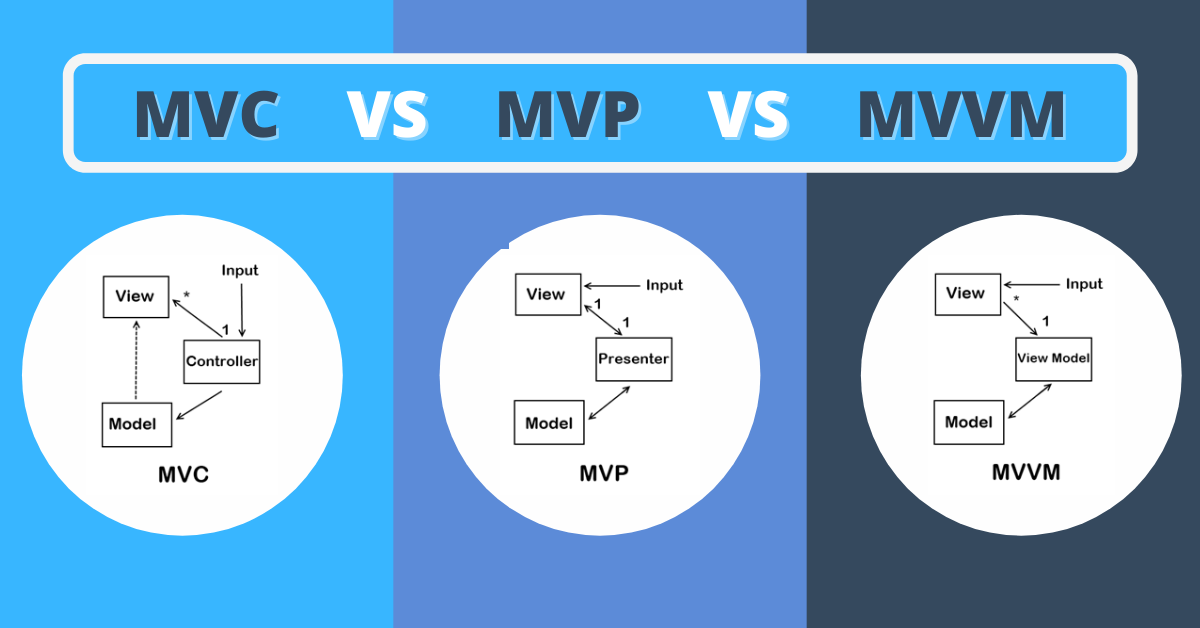
\includegraphics[width=0.9\textwidth]{figure1.png}
\caption{MVC vs MVP vs MVVM.}
\label{fig:1}
\end{figure}

\newpage
\hspace{0pt} %

\end{document}
